\documentclass{article}

\usepackage{a4}
\usepackage{setspace}
\usepackage{graphicx}
\usepackage{amsmath}
\usepackage[version = 4]{mhchem}
\usepackage{hyperref}
\usepackage{float}


\setlength{\parindent}{0pt}

\title{A Deeper Understanding of the s-Process:\\
A Ph.D. Oral Qualifier}
\author{by: Jaad A. Tannous\\
Advisor: Prof. Bradley S. Meyer}
\date{}

\begin{document}
\maketitle

\section*{Abstract}
The aim of this document is to provide the committee a brief layout of the aspects that will comprise my dissertation. The first 
section is a brief recap, but granted not a complete one, on the s-process. The following four will outline aspects of the s-process 
that are of interest. The final one describes how it all comes together

\section*{The s-process}
The slow neutron capture process, s-process, is a series of reactions in nuclear astrophysics that is responsible 
for synthesizing half the elements heavier than Iron. It occurs in moderately neutron rich environments and requires 
existing Iron as a seed nucleus. The reactions involved are a series of neutron captures and $\beta^{-}$ decays. Heavier 
isotopes will form until one that is $\beta$ unstable is reached, and its decay rate is higher than the capture rate; as illustrated 
in Fig. \ref{fig 1}.

\begin{figure}[!htp]
    \centerline{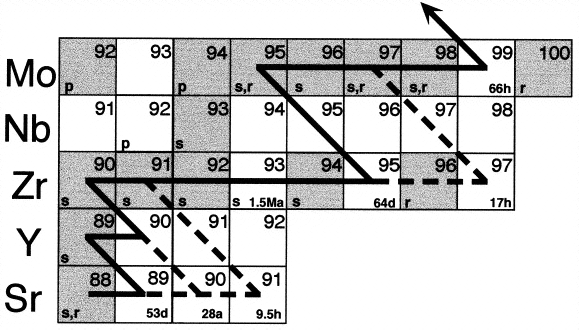
\includegraphics[scale = 0.5]{images/sprocess.png}}
    \caption{A Z-N flow chart illustrating a cut of s-process nucleosynthesis from Strontium up till 
    Molybdenum. The solid line indicates the main path, while the dotted a secondary branch \cite{nic98}.}
    \label{fig 1}
\end{figure}

 It is a slow process because the $\beta^{-}$ decays occur on shorter timescales than the next neutron capture. In comparison, 
neutron captures may take days or years, while beta decays can take between seconds and hours.\\

 S-process nucleosynthesis occur in two types of stars; during Thermal Pulsing Asymptotic Giant Branch stars, TP-AGB, and massive stars 
have achieved core Helium burning and beyond. The s-process yields and branching extent are affected by two major factors. The first being the 
star's capability to generate neutrons. The second being the amount of Iron the star was able to accrete from the cloud it formed from.\\

 The yields and end products generated by TP-AGB stars and massive stars are so different, they are categorized into main branch and weak 
branch s-process. The main branch s-process nucleosynthesis occurs in TP-AGB stars, specifically in low mass stars. It produces heavy 
elements up to Lead in low metallicity stars. In this phase, neutron source is $^{13}C$ created during the third dredge up \cite{kww} and 
produces neutrons via:

\begin{equation*}
\ce{^13C + ^4He -> ^16O + n} 
\end{equation*}

 The weak s-process branch occurs at the end of core Helium and Carbon burning in massive stars. It produces heavy elements up Yttrium.
The element that will supply the neutron is the isotope $^{22}Ne$ via:

\begin{equation*}
    \ce{^22Ne + ^4He -> ^25Mg + n}
\end{equation*}

 Due to low neutron fluxes, $10^{5}$ to $10^{11} cm^{-2}s^{-1}$, the s-process cannot produce the heavy radioactive such as Uranium. 
However, it terminates in a Bismuth, Lead, Polonium loop:

\begin{align*}
    \ce{^209Bi + n &-> ^210Bi + \gamma}\\
    \ce{^210Bi &-> ^210Po + e^- + \bar{\nu_{e}}}\\
    \ce{^210Po &-> ^206Pb + ^4He}\\
    \ce{^206Pb + 3n &-> ^209Pb}\\
    \ce{^209Pb &-> ^209Bi + e^- + \bar{\nu_{e}}}
\end{align*}

\section*{Neutron Exposure}

For a given species `i' whose only interaction is neutron capture, its total abundance over time is governed by:

\begin{align*}
    \frac{d Y_{i}}{dt} &= -N_{A}\left<\sigma v\right>\rho Y_{i}Y_{n}\\
    \frac{d Y_{i}}{dt} &= -n_{n} \left<\sigma v\right> Y_{i}
\end{align*}

The differential exposure and neutron capture cross-section are respectively given by:
\begin{align*}
    d\tau &= n_{n}v_{T}dt\\
    \sigma_{i} &= \frac{\left<\sigma v\right>}{v_{T}}
\end{align*}

Where $n_{n}$ is the neutron number density and $v_{T}$ is the thermal velocity of neutrons. The first order differential equation 
now becomes

\begin{equation*}
    \frac{d Y_{i}}{d\tau} = -\sigma_{i}Y_{i}
\end{equation*}
And has a solution
\begin{equation*}
    Y_{i}(\tau) = Y_{i}(0)e^{-\sigma_{i}\tau}
\end{equation*}

Realistically, we always have an ensemble of species with unique cross-sections. Such an ensemble requires the introduction  of a 
normalized density of exposures $\rho(\tau)$. The solution of the above ODE generalizes to:

\begin{equation*}
    Y_{i}(\tau) = Y_i(0)\int_{0}^{\infty}\rho(\tau)e^{-\sigma_{i}\tau}d\tau
\end{equation*}

Generally speaking, $\rho(\tau)$ is unknown and must be solved for. An exponential distribution of exposures was suggested \cite{clayton1974s}, 
however it is specific to certain mixing models. With additional mixing processes induced by rotation and magnetic fields, a 
general form for the density of exposures is necessary. Upon closer inspection, we realize that

\begin{equation*}
    \frac{Y_{i}(\tau)}{Y_i(0)} = \int_{0}^{\infty}\rho(\tau)e^{-\sigma_{i}\tau}d\tau = \tilde{\rho}(\sigma_{i})
\end{equation*}

Where $\tilde{\rho}$ is the Laplace transform of the exposure density into cross-section space, which is easily attainable using 
libnucnet \cite{meyer}. The exercise becomes solving for the inverse Laplace transform in post-processing. Formally, the inverse 
Laplace transform is determined by the Bromwich integral:

\begin{equation*}
    \rho(\tau) = \frac{1}{2\pi i} \lim_{T\to\infty}\int_{\gamma - iT}^{\gamma + iT}e^{\sigma_{i}\tau}\tilde{\rho}(\sigma_{i})
\end{equation*}

Which is a line integral in the complex plane. Without having an analytical form for $\tilde{\rho}$, solving the integral with standard 
procedures, such as Cauchy Residue theorem, is quite challenging numerically. To circumvent said challenge, we apply the Gaver-Stehfest (GS) 
method \cite{jacquot1983gaver}. In short the method transforms the integral into the real plane and suggests an appropriate discretization. 
Figures \ref{fig 2} and \ref{fig 3} show the method's effectiveness at approximating the inverse, where the analytical forms are known. 
The Jupyter notebook used to generate the graphs is found \href{https://github.com/jaadt7/gaver_stehfest}{here}. The notebook itself goes through 
exponential, Poisson, and Gaussian distributions; showing the method's effectiveness on each.

\begin{figure}[!htp]
    \centerline{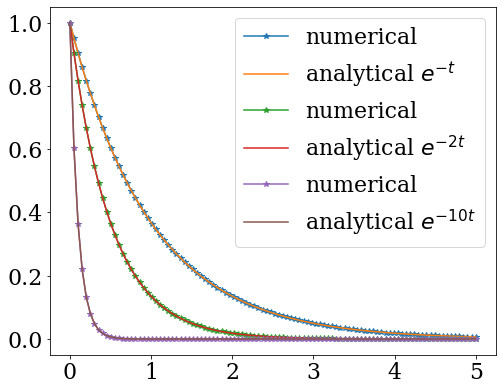
\includegraphics[scale = 0.5]{images/exp_test_1.png}}
    \caption{Testing the Gaver-Stehfest method on decaying exponential functions}
    \label{fig 2}
\end{figure}

\begin{figure}[!htp]
    \centerline{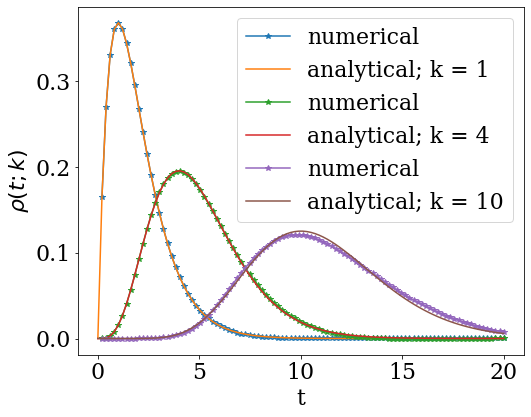
\includegraphics[scale = 0.5]{images/poisson_test.png}}
    \caption{Testing the Gaver-Stehfest method various Poisson distributions}
    \label{fig 3}
\end{figure}


Building the testing environment involved setting up the multi-zone version of the network with s-process like conditions and artificial 
species with user defined cross-sections. Based on the discretization scheme provided by the GS method, we developed an algorithm 
that creates the appropriate amount of "dummy" species with specified neutron capture cross-sections. The species were loaded into the 
multi-zone code, and the GS method was applied iteratively on the output. Animations were used to visualize the time 
evolution of the density of exposures 

\section*{Isomers}

s-Process calculations can take various routes to reach its terminal loop. The branching of the s-process depends on a multitude of 
conditions, one of which is the isomeric state of a given isotope. The isomeric state of a given species has a $\beta$-decay rate 
orders of magnitude higher than that of the ground state. In collaboration with Los Alamos [insert citation], we focus on the 
effect of isomeric $^{85}$Kr, since it is a pivoting isotope. To build some understanding on how the isomers may build up in a system, 
I developed a simplistic two-species network found \href{https://github.com/jaadt7/isomer_intuition}{here}.
The two species involved are the meta-stable, isomeric, and ground states of $^{85}$Kr.\\ 

The equations being modeled are:

\begin{align*}
    \ce{^85Kr_g + \gamma &-> ^85Kr_m}\\
    \ce{^85Kr_m + \gamma &-> ^85Kr_g}
\end{align*}

Figure \ref{rates} shows that in the low temperature regime, the evolution of the system will be towards the ground state. As the 
temperature increases, the system should reach some equilibrium between the two. The decay rate used is from the JINA reaction 
library [citation needed], while the excitation rate is calculated from the reverse rate in combination with the ground and 
isomeric ensemble partition functions.


\begin{figure}[H]
    \centerline{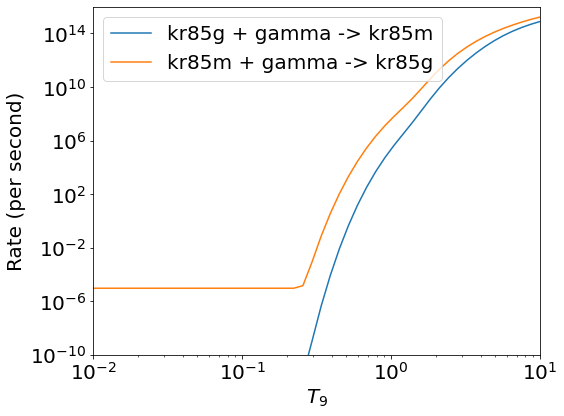
\includegraphics[scale = 0.5]{images/iso_rates.png}}
    \caption{Reaction rates as a function of $T_{9}$ for excitation and de-exitation of $^{85}Kr$}
    \label{rates}
\end{figure}

The temperature evolution chosen is a simple oscillatory profile that mimics the temperature fluctuations during the TP-AGB phase but 
on a shorter time scale, see Fig \ref{temp}. This temperature range places the reaction rates in the central region of Fig. \ref{rates}.

\begin{figure}[H]
    \centerline{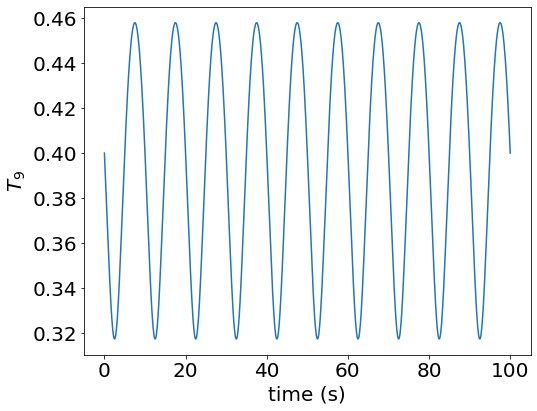
\includegraphics[scale = 0.5]{images/temp_profile.png}}
    \caption{Temperature profile as a function of time, $T_{9}(t=0)$ = 0.4, oscillating over a 10s period}
    \label{temp}
\end{figure}

The evolution of $X(^{85}Kr_{m})$ is described in figure \ref{mfrac}. The orange stars represent the equilibrium mass fraction, calculated 
via Boltzmann statistics, and the blue curve is the network calculation.

\begin{figure}[H]
    \centerline{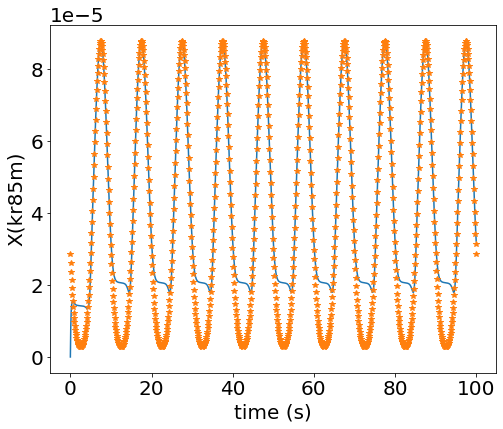
\includegraphics[scale = 0.5]{images/mass_frac.png}}
    \caption{The evolution of $X(^{85}Kr_{m})$ and the $X(^{85}Kr_{m})_{eq}$ as a function of time}
    \label{mfrac}
\end{figure}

Ideally, mass fraction would evolve along the equilibrium value, and for the most part, it does. However, as the temperature drops, 
the exchange between the two states freezes the abundance. When the temperature is back on the rise, the mass fraction tends back to 
the equilibrium value and catches up to it. The rate is high enough that the abundance keeps up with the equilibrium value.\\

\begin{figure}[H]
    \centerline{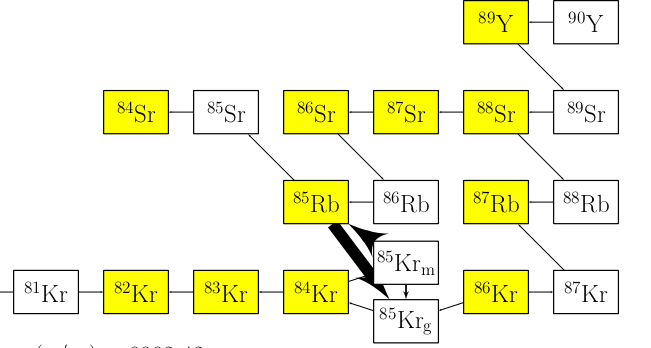
\includegraphics[scale = 0.5]{images/sample_branch.png}}
    \caption{The difference of integrated currents between the cases of when the isomer was taken into account and when it all decayed to the ground state}
    \label{int_cur}
\end{figure}

For proper network calculations, our collaborators have supplied us with structural and compositional data. This data is generated 
by evolving a 2 $M_{\odot}$ star with Z = 0.02 going through the TP-AGB phase with the MESA code [version needed]\cite{paxton2010modules,paxton2013modules,paxton2015modules,paxton2018modules,paxton2019modules}.
The structural data comprises 5 mass coordinates, covering the extent of the $^{13}$C pocket, along with the temperature and density 
of those coordinates over time. Libnucnet was run along these trajectories twice, once with the reactions pertaining to $^{85}$Kr$_{m}$ 
and the other without the isomer. This was done on palmetto in parallel for multiple temperature scales for each mass 
coordinate trajectory.\\

Fig. \ref{int_cur} shows a sampling of the performed calculations. It is a flow diagram of integrated currents centered at $^{85}$Kr. 
This particular calculation was done at the lowest mass coordinate which has the highest temperature profile of them all. To be more 
specific, the flow chart is in fact a difference of integrated currents at the end of the simulation. It is subtracting the current 
due to the modified network from the unmodified network. That is why the arrow is pointing from $^{85}$Rb down to $^{85}$Kr. It 
also illustrates why $^{85}$Kr is a pivoting point. The meta-stable state allows the build up to Strontium through, $^{85}$Sr, while 
neglecting it results in Strontium building up through $^{88}$Sr. Accounting for isomers in network calculations might help explain 
the enhanced observed abundance of lighter stable isotopes.

\section*{T and $Y_{e}$ dependent rates}

During the s-process, neutron rich isotopes might be synthesized via electron capture. The rates of these weak interactions, weak rates, 
are not in fact solely dependent on density and temperature, but on the electron mass fraction, Y$_{e}$, as well.

\begin{figure}[H]
    \centerline{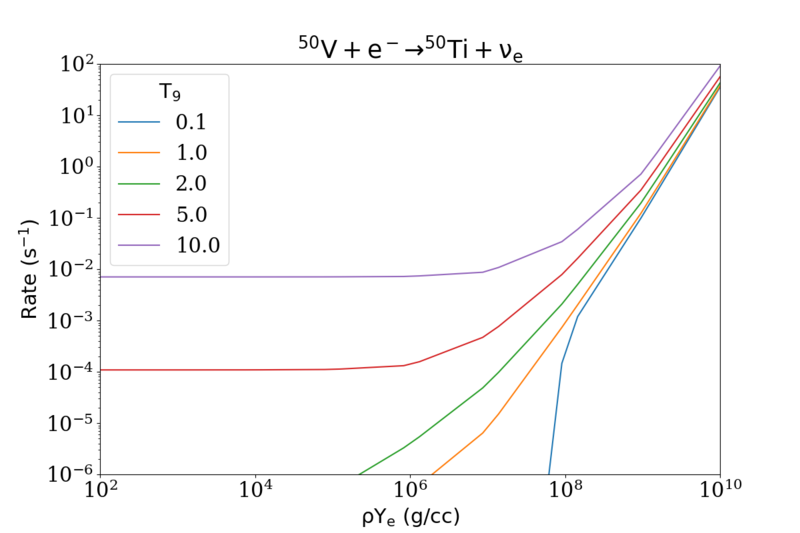
\includegraphics[scale = 0.5]{images/van_weak.png}}
    \caption{The variation of the weak rate of $^{50}$V as a function of $\rho$Y$_{e}$ at constant temperature}
    \label{weak}
\end{figure}

Figure \ref{weak} illustrates $^{50}$V's weak rate's dependency on Y$_{e}$. The drastic change in behavior the rate displays for a 
given Y$_{e}$ across the temperature range, especially at the lower end, suggests that the effect should not be neglected. To focus 
on more s-process related species, we focus on $^{205}$Pb; which is exclusively produced by it. With a half-life of about 17 Myr, 
it decays into $^{205}$Tl via:

\begin{align*}
    \ce{^205Pb + e^- -> ^205Tl + \nu_{e}}
\end{align*}

Another reason for using $^{205}$Pb is for studying the early solar system. Analysis of Thallium within carbonaceous chondrites
has lead to believe that $^{205}$Pb existed in the early solar system \cite{baker2010thallium}.

\section*{Multi-zone framework development}

Understanding stellar structure requires visual aids to strengthen one's intuition and verify their assumptions. Kippenhahn diagrams 
are one such example. Kippenhahn diagrams are used to show convective regions in a stellar environment over a given length of time, see
fig. \ref{conv}

\begin{figure}[H]
    \centerline{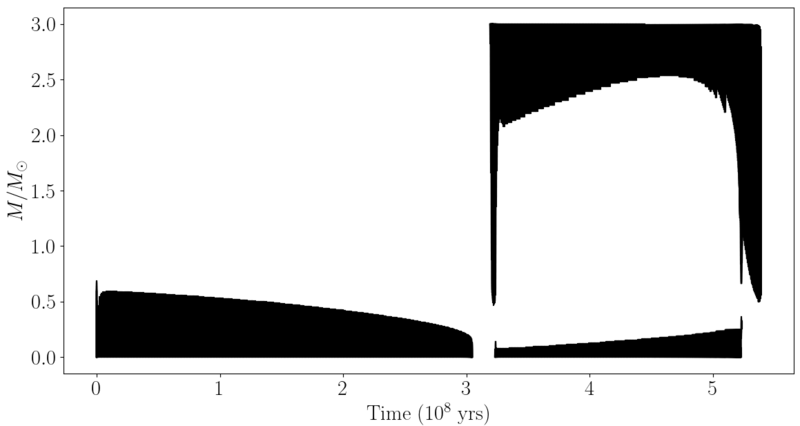
\includegraphics[scale = 0.5]{images/conv.png}}
    \caption{The convective profile of a 3$M_{\odot}$ star from ZAMS till the TP-AGB phase}
    \label{conv}
\end{figure}

These diagrams are generated by graphing the extent of the convective region in terms of mass coordinate in each time step. Simply 
put, it is a collection of vertical lines graphed at a given timestep. The aim here is to extend the application of these diagrams 
to illustrate the evolution of other properties such as temperature. Fig \ref{movie_cut} depicts precisely that.

\begin{figure}[H]
    \centerline{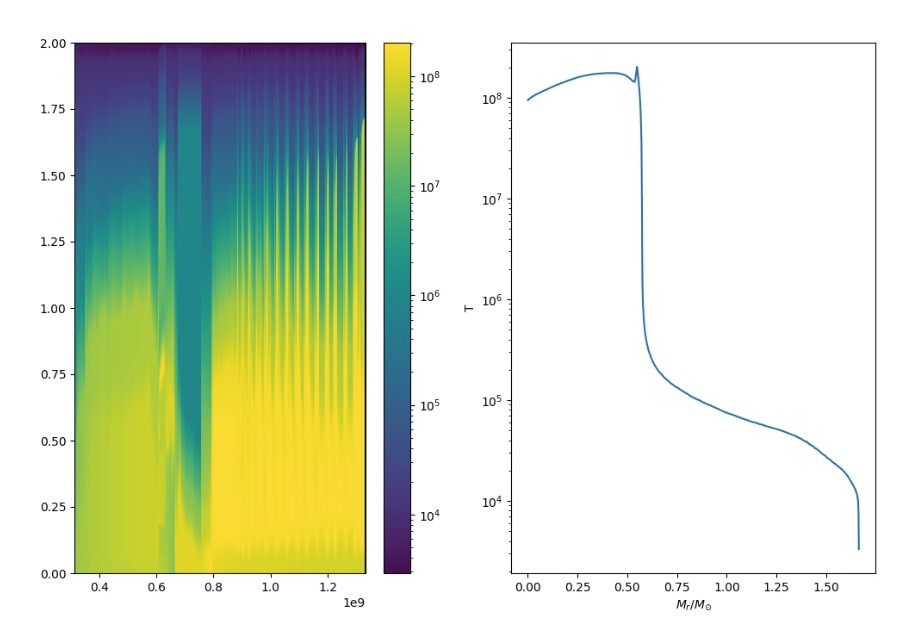
\includegraphics[scale = 0.5]{images/movie_slice.png}}
    \caption{A snapshot of the animation that shows a static color map of the temperature profile over time with a black vertical 
    line which indicates the current timestamp of interest and the temperature profile of the star at that time stamp as a function 
    of mass coordinate. The star here is 2 $M_{\odot}$.}
    \label{movie_cut}
\end{figure}

The figure on the left has the same axes as a Kippenhahn diagram, but instead of showing the extent of a convective zone, it shows 
the temperature value with a color map scale. The same could be done for other properties of interest, such as density, diffusion 
coefficients, or even mass fractions of species of interest. The current downside of the method is the amount of converged stellar 
models available in a saved file. To remedy this, a 2D interpolator is being developed to smoothly to pad with appropriate 
approximations. More converged models could be saved, but it is avoided for memory purposes. The color map utility allows for a 
smooth global analysis of a given property.

\section*{Piecing it all together}

To study outlined aspects, we have to look what goes on in the s-process' ``natural habitat". As illustrated in my masters thesis, rotation 
has major effects on the various phases of stellar evolution. The rotationally induced mixing modes are of specific interest. The study 
will be carried out by first marrying libnucnet to the stellar evolution code, then evolving stars to the phases where s-process occurs. 
This will feed the nuclear network with real-time stellar temperature, density, and mixing profiles so s-process calculations can be 
carried out under more realistic conditions. The post-processing tools would then be used to analyze the output generated by the union 
and conclusions would be drawn from there.

\singlespacing

\bibliographystyle{unsrt}
\bibliography{references.bib}

\end{document}